\documentclass[tikz,12pt,border=2pt]{standalone}
\usepackage[T1]{fontenc}
\usepackage[scaled=0.92]{helvet}
\renewcommand{\familydefault}{\sfdefault}
\usetikzlibrary{calc,patterns}
\definecolor{cexf}{RGB}{31,84,140}
\definecolor{cimp}{RGB}{179,38,30}
\definecolor{cdex}{RGB}{168,116,26}
\definecolor{cnon}{RGB}{111,78,156}
\definecolor{cagg}{RGB}{58,125,68}
\definecolor{cbase}{RGB}{122,122,122}
\definecolor{cmov}{RGB}{31,84,140}
\begin{document}
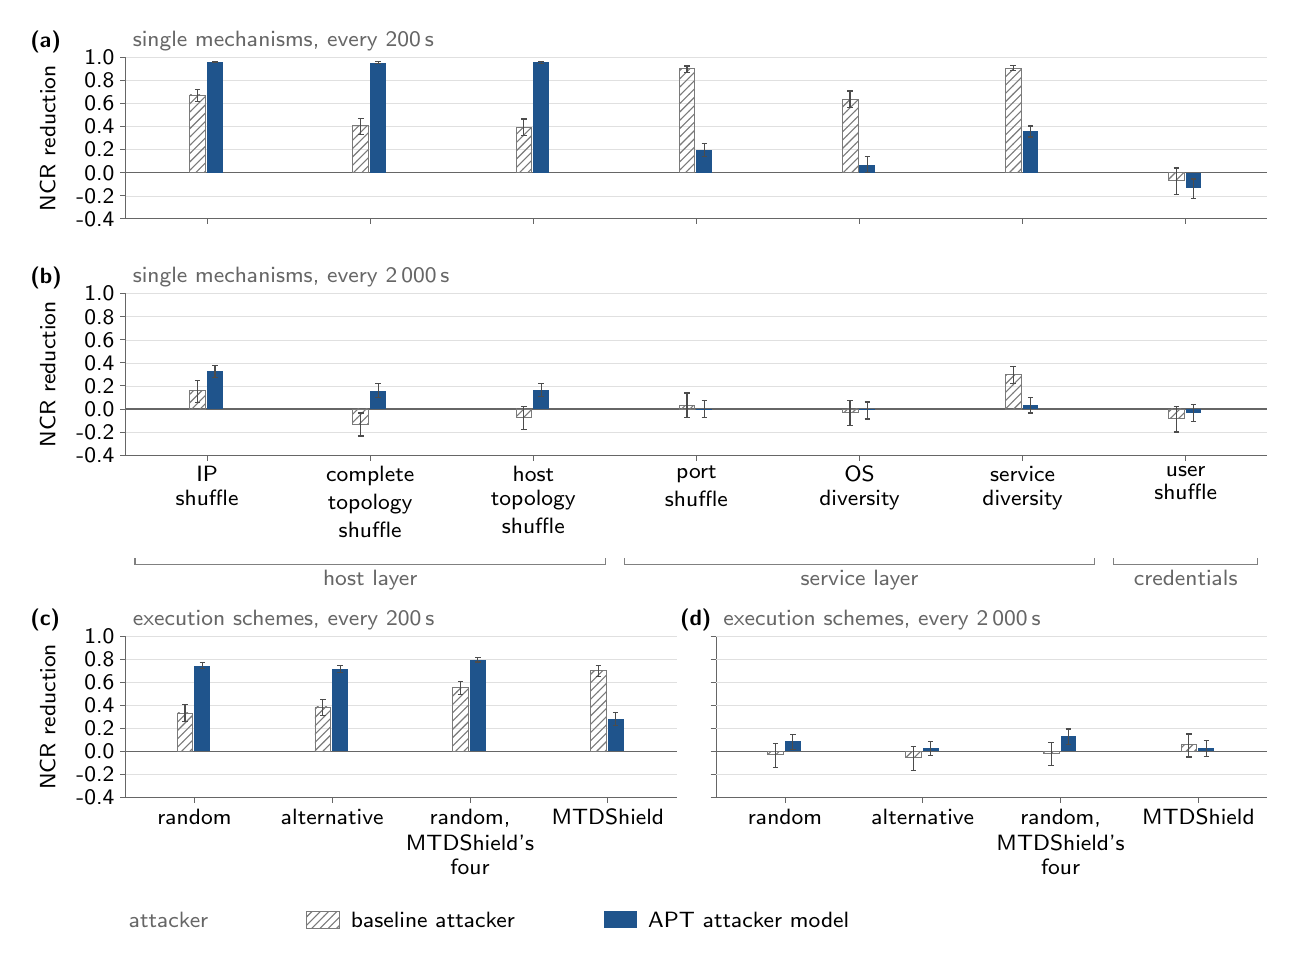
\begin{tikzpicture}[x=1cm,y=1cm,every node/.style={inner sep=1pt,font=\footnotesize}]
\draw[black!60,line width=0.4pt] (1.300,9.150) -- (15.800,9.150);
\draw[black!60,line width=0.4pt] (1.300,9.150) -- (1.300,11.200);
\draw[black!60,line width=0.3pt] (1.230,9.150) -- (1.300,9.150);
\node[anchor=east] at (1.200,9.150) {-0.4};
\draw[black!60,line width=0.3pt] (1.230,9.443) -- (1.300,9.443);
\draw[black!12,line width=0.2pt] (1.300,9.443) -- (15.800,9.443);
\node[anchor=east] at (1.200,9.443) {-0.2};
\draw[black!60,line width=0.3pt] (1.230,9.736) -- (1.300,9.736);
\draw[black!12,line width=0.2pt] (1.300,9.736) -- (15.800,9.736);
\node[anchor=east] at (1.200,9.736) {0.0};
\draw[black!60,line width=0.3pt] (1.230,10.029) -- (1.300,10.029);
\draw[black!12,line width=0.2pt] (1.300,10.029) -- (15.800,10.029);
\node[anchor=east] at (1.200,10.029) {0.2};
\draw[black!60,line width=0.3pt] (1.230,10.321) -- (1.300,10.321);
\draw[black!12,line width=0.2pt] (1.300,10.321) -- (15.800,10.321);
\node[anchor=east] at (1.200,10.321) {0.4};
\draw[black!60,line width=0.3pt] (1.230,10.614) -- (1.300,10.614);
\draw[black!12,line width=0.2pt] (1.300,10.614) -- (15.800,10.614);
\node[anchor=east] at (1.200,10.614) {0.6};
\draw[black!60,line width=0.3pt] (1.230,10.907) -- (1.300,10.907);
\draw[black!12,line width=0.2pt] (1.300,10.907) -- (15.800,10.907);
\node[anchor=east] at (1.200,10.907) {0.8};
\draw[black!60,line width=0.3pt] (1.230,11.200) -- (1.300,11.200);
\draw[black!12,line width=0.2pt] (1.300,11.200) -- (15.800,11.200);
\node[anchor=east] at (1.200,11.200) {1.0};
\node[rotate=90,anchor=south] at (0.450,10.175) {NCR reduction};
\draw[black!60,line width=0.3pt] (2.336,9.150) -- (2.336,9.080);
\draw[black!60,line width=0.3pt] (4.407,9.150) -- (4.407,9.080);
\draw[black!60,line width=0.3pt] (6.479,9.150) -- (6.479,9.080);
\draw[black!60,line width=0.3pt] (8.550,9.150) -- (8.550,9.080);
\draw[black!60,line width=0.3pt] (10.621,9.150) -- (10.621,9.080);
\draw[black!60,line width=0.3pt] (12.693,9.150) -- (12.693,9.080);
\draw[black!60,line width=0.3pt] (14.764,9.150) -- (14.764,9.080);
\draw[black!60,line width=0.4pt] (1.300,9.736) -- (15.800,9.736);
\node[anchor=south west,font=\footnotesize\bfseries] at (0.050,11.220) {(a)};
\node[anchor=south west,text=black!60] at (1.350,11.240) {single mechanisms, every 200\,s};
\fill[pattern=north east lines,pattern color=cbase] (2.116,9.736) rectangle (2.316,10.724);
\draw[cbase,line width=0.3pt] (2.116,9.736) rectangle (2.316,10.724);
\draw[black!70,line width=0.4pt] (2.216,10.644) -- (2.216,10.795);
\draw[black!70,line width=0.4pt] (2.181,10.644) -- (2.251,10.644);
\draw[black!70,line width=0.4pt] (2.181,10.795) -- (2.251,10.795);
\fill[cmov] (2.336,9.736) rectangle (2.536,11.143);
\draw[black!70,line width=0.4pt] (2.436,11.132) -- (2.436,11.154);
\draw[black!70,line width=0.4pt] (2.401,11.132) -- (2.471,11.132);
\draw[black!70,line width=0.4pt] (2.401,11.154) -- (2.471,11.154);
\fill[pattern=north east lines,pattern color=cbase] (4.187,9.736) rectangle (4.387,10.331);
\draw[cbase,line width=0.3pt] (4.187,9.736) rectangle (4.387,10.331);
\draw[black!70,line width=0.4pt] (4.287,10.225) -- (4.287,10.428);
\draw[black!70,line width=0.4pt] (4.252,10.225) -- (4.322,10.225);
\draw[black!70,line width=0.4pt] (4.252,10.428) -- (4.322,10.428);
\fill[cmov] (4.407,9.736) rectangle (4.607,11.134);
\draw[black!70,line width=0.4pt] (4.507,11.121) -- (4.507,11.146);
\draw[black!70,line width=0.4pt] (4.472,11.121) -- (4.542,11.121);
\draw[black!70,line width=0.4pt] (4.472,11.146) -- (4.542,11.146);
\fill[pattern=north east lines,pattern color=cbase] (6.259,9.736) rectangle (6.459,10.315);
\draw[cbase,line width=0.3pt] (6.259,9.736) rectangle (6.459,10.315);
\draw[black!70,line width=0.4pt] (6.359,10.208) -- (6.359,10.418);
\draw[black!70,line width=0.4pt] (6.324,10.208) -- (6.394,10.208);
\draw[black!70,line width=0.4pt] (6.324,10.418) -- (6.394,10.418);
\fill[cmov] (6.479,9.736) rectangle (6.679,11.137);
\draw[black!70,line width=0.4pt] (6.579,11.126) -- (6.579,11.148);
\draw[black!70,line width=0.4pt] (6.544,11.126) -- (6.614,11.126);
\draw[black!70,line width=0.4pt] (6.544,11.148) -- (6.614,11.148);
\fill[pattern=north east lines,pattern color=cbase] (8.330,9.736) rectangle (8.530,11.056);
\draw[cbase,line width=0.3pt] (8.330,9.736) rectangle (8.530,11.056);
\draw[black!70,line width=0.4pt] (8.430,11.013) -- (8.430,11.092);
\draw[black!70,line width=0.4pt] (8.395,11.013) -- (8.465,11.013);
\draw[black!70,line width=0.4pt] (8.395,11.092) -- (8.465,11.092);
\fill[cmov] (8.550,9.736) rectangle (8.750,10.027);
\draw[black!70,line width=0.4pt] (8.650,9.939) -- (8.650,10.111);
\draw[black!70,line width=0.4pt] (8.615,9.939) -- (8.685,9.939);
\draw[black!70,line width=0.4pt] (8.615,10.111) -- (8.685,10.111);
\fill[pattern=north east lines,pattern color=cbase] (10.401,9.736) rectangle (10.601,10.672);
\draw[cbase,line width=0.3pt] (10.401,9.736) rectangle (10.601,10.672);
\draw[black!70,line width=0.4pt] (10.501,10.569) -- (10.501,10.774);
\draw[black!70,line width=0.4pt] (10.466,10.569) -- (10.536,10.569);
\draw[black!70,line width=0.4pt] (10.466,10.774) -- (10.536,10.774);
\fill[cmov] (10.621,9.736) rectangle (10.821,9.838);
\draw[black!70,line width=0.4pt] (10.721,9.739) -- (10.721,9.937);
\draw[black!70,line width=0.4pt] (10.686,9.739) -- (10.756,9.739);
\draw[black!70,line width=0.4pt] (10.686,9.937) -- (10.756,9.937);
\fill[pattern=north east lines,pattern color=cbase] (12.473,9.736) rectangle (12.673,11.065);
\draw[cbase,line width=0.3pt] (12.473,9.736) rectangle (12.673,11.065);
\draw[black!70,line width=0.4pt] (12.573,11.031) -- (12.573,11.095);
\draw[black!70,line width=0.4pt] (12.538,11.031) -- (12.608,11.031);
\draw[black!70,line width=0.4pt] (12.538,11.095) -- (12.608,11.095);
\fill[cmov] (12.693,9.736) rectangle (12.893,10.263);
\draw[black!70,line width=0.4pt] (12.793,10.190) -- (12.793,10.329);
\draw[black!70,line width=0.4pt] (12.758,10.190) -- (12.828,10.190);
\draw[black!70,line width=0.4pt] (12.758,10.329) -- (12.828,10.329);
\fill[pattern=north east lines,pattern color=cbase] (14.544,9.638) rectangle (14.744,9.736);
\draw[cbase,line width=0.3pt] (14.544,9.638) rectangle (14.744,9.736);
\draw[black!70,line width=0.4pt] (14.644,9.464) -- (14.644,9.796);
\draw[black!70,line width=0.4pt] (14.609,9.464) -- (14.679,9.464);
\draw[black!70,line width=0.4pt] (14.609,9.796) -- (14.679,9.796);
\fill[cmov] (14.764,9.538) rectangle (14.964,9.736);
\draw[black!70,line width=0.4pt] (14.864,9.407) -- (14.864,9.656);
\draw[black!70,line width=0.4pt] (14.829,9.407) -- (14.899,9.407);
\draw[black!70,line width=0.4pt] (14.829,9.656) -- (14.899,9.656);
\draw[black!60,line width=0.4pt] (1.300,6.150) -- (15.800,6.150);
\draw[black!60,line width=0.4pt] (1.300,6.150) -- (1.300,8.200);
\draw[black!60,line width=0.3pt] (1.230,6.150) -- (1.300,6.150);
\node[anchor=east] at (1.200,6.150) {-0.4};
\draw[black!60,line width=0.3pt] (1.230,6.443) -- (1.300,6.443);
\draw[black!12,line width=0.2pt] (1.300,6.443) -- (15.800,6.443);
\node[anchor=east] at (1.200,6.443) {-0.2};
\draw[black!60,line width=0.3pt] (1.230,6.736) -- (1.300,6.736);
\draw[black!12,line width=0.2pt] (1.300,6.736) -- (15.800,6.736);
\node[anchor=east] at (1.200,6.736) {0.0};
\draw[black!60,line width=0.3pt] (1.230,7.029) -- (1.300,7.029);
\draw[black!12,line width=0.2pt] (1.300,7.029) -- (15.800,7.029);
\node[anchor=east] at (1.200,7.029) {0.2};
\draw[black!60,line width=0.3pt] (1.230,7.321) -- (1.300,7.321);
\draw[black!12,line width=0.2pt] (1.300,7.321) -- (15.800,7.321);
\node[anchor=east] at (1.200,7.321) {0.4};
\draw[black!60,line width=0.3pt] (1.230,7.614) -- (1.300,7.614);
\draw[black!12,line width=0.2pt] (1.300,7.614) -- (15.800,7.614);
\node[anchor=east] at (1.200,7.614) {0.6};
\draw[black!60,line width=0.3pt] (1.230,7.907) -- (1.300,7.907);
\draw[black!12,line width=0.2pt] (1.300,7.907) -- (15.800,7.907);
\node[anchor=east] at (1.200,7.907) {0.8};
\draw[black!60,line width=0.3pt] (1.230,8.200) -- (1.300,8.200);
\draw[black!12,line width=0.2pt] (1.300,8.200) -- (15.800,8.200);
\node[anchor=east] at (1.200,8.200) {1.0};
\draw[black!60,line width=0.3pt] (2.336,6.150) -- (2.336,6.080);
\node[anchor=north] at (2.336,6.050) {\shortstack{IP\\shuffle}};
\draw[black!60,line width=0.3pt] (4.407,6.150) -- (4.407,6.080);
\node[anchor=north] at (4.407,6.050) {\shortstack{complete\\topology\\shuffle}};
\draw[black!60,line width=0.3pt] (6.479,6.150) -- (6.479,6.080);
\node[anchor=north] at (6.479,6.050) {\shortstack{host\\topology\\shuffle}};
\draw[black!60,line width=0.3pt] (8.550,6.150) -- (8.550,6.080);
\node[anchor=north] at (8.550,6.050) {\shortstack{port\\shuffle}};
\draw[black!60,line width=0.3pt] (10.621,6.150) -- (10.621,6.080);
\node[anchor=north] at (10.621,6.050) {\shortstack{OS\\diversity}};
\draw[black!60,line width=0.3pt] (12.693,6.150) -- (12.693,6.080);
\node[anchor=north] at (12.693,6.050) {\shortstack{service\\diversity}};
\draw[black!60,line width=0.3pt] (14.764,6.150) -- (14.764,6.080);
\node[anchor=north] at (14.764,6.050) {\shortstack{user\\shuffle}};
\node[rotate=90,anchor=south] at (0.450,7.175) {NCR reduction};
\draw[black!60,line width=0.4pt] (1.300,6.736) -- (15.800,6.736);
\node[anchor=south west,font=\footnotesize\bfseries] at (0.050,8.220) {(b)};
\node[anchor=south west,text=black!60] at (1.350,8.240) {single mechanisms, every 2\,000\,s};
\fill[pattern=north east lines,pattern color=cbase] (2.116,6.736) rectangle (2.316,6.967);
\draw[cbase,line width=0.3pt] (2.116,6.736) rectangle (2.316,6.967);
\draw[black!70,line width=0.4pt] (2.216,6.817) -- (2.216,7.101);
\draw[black!70,line width=0.4pt] (2.181,6.817) -- (2.251,6.817);
\draw[black!70,line width=0.4pt] (2.181,7.101) -- (2.251,7.101);
\fill[cmov] (2.336,6.736) rectangle (2.536,7.214);
\draw[black!70,line width=0.4pt] (2.436,7.131) -- (2.436,7.292);
\draw[black!70,line width=0.4pt] (2.401,7.131) -- (2.471,7.131);
\draw[black!70,line width=0.4pt] (2.401,7.292) -- (2.471,7.292);
\fill[pattern=north east lines,pattern color=cbase] (4.187,6.544) rectangle (4.387,6.736);
\draw[cbase,line width=0.3pt] (4.187,6.544) rectangle (4.387,6.736);
\draw[black!70,line width=0.4pt] (4.287,6.392) -- (4.287,6.685);
\draw[black!70,line width=0.4pt] (4.252,6.392) -- (4.322,6.392);
\draw[black!70,line width=0.4pt] (4.252,6.685) -- (4.322,6.685);
\fill[cmov] (4.407,6.736) rectangle (4.607,6.970);
\draw[black!70,line width=0.4pt] (4.507,6.876) -- (4.507,7.056);
\draw[black!70,line width=0.4pt] (4.472,6.876) -- (4.542,6.876);
\draw[black!70,line width=0.4pt] (4.472,7.056) -- (4.542,7.056);
\fill[pattern=north east lines,pattern color=cbase] (6.259,6.631) rectangle (6.459,6.736);
\draw[cbase,line width=0.3pt] (6.259,6.631) rectangle (6.459,6.736);
\draw[black!70,line width=0.4pt] (6.359,6.474) -- (6.359,6.767);
\draw[black!70,line width=0.4pt] (6.324,6.474) -- (6.394,6.474);
\draw[black!70,line width=0.4pt] (6.324,6.767) -- (6.394,6.767);
\fill[cmov] (6.479,6.736) rectangle (6.679,6.980);
\draw[black!70,line width=0.4pt] (6.579,6.891) -- (6.579,7.065);
\draw[black!70,line width=0.4pt] (6.544,6.891) -- (6.614,6.891);
\draw[black!70,line width=0.4pt] (6.544,7.065) -- (6.614,7.065);
\fill[pattern=north east lines,pattern color=cbase] (8.330,6.736) rectangle (8.530,6.781);
\draw[cbase,line width=0.3pt] (8.330,6.736) rectangle (8.530,6.781);
\draw[black!70,line width=0.4pt] (8.430,6.627) -- (8.430,6.939);
\draw[black!70,line width=0.4pt] (8.395,6.627) -- (8.465,6.627);
\draw[black!70,line width=0.4pt] (8.395,6.939) -- (8.465,6.939);
\fill[cmov] (8.550,6.736) rectangle (8.750,6.739);
\draw[black!70,line width=0.4pt] (8.650,6.629) -- (8.650,6.844);
\draw[black!70,line width=0.4pt] (8.615,6.629) -- (8.685,6.629);
\draw[black!70,line width=0.4pt] (8.615,6.844) -- (8.685,6.844);
\fill[pattern=north east lines,pattern color=cbase] (10.401,6.698) rectangle (10.601,6.736);
\draw[cbase,line width=0.3pt] (10.401,6.698) rectangle (10.601,6.736);
\draw[black!70,line width=0.4pt] (10.501,6.528) -- (10.501,6.845);
\draw[black!70,line width=0.4pt] (10.466,6.528) -- (10.536,6.528);
\draw[black!70,line width=0.4pt] (10.466,6.845) -- (10.536,6.845);
\fill[cmov] (10.621,6.721) rectangle (10.821,6.736);
\draw[black!70,line width=0.4pt] (10.721,6.608) -- (10.721,6.824);
\draw[black!70,line width=0.4pt] (10.686,6.608) -- (10.756,6.608);
\draw[black!70,line width=0.4pt] (10.686,6.824) -- (10.756,6.824);
\fill[pattern=north east lines,pattern color=cbase] (12.473,6.736) rectangle (12.673,7.173);
\draw[cbase,line width=0.3pt] (12.473,6.736) rectangle (12.673,7.173);
\draw[black!70,line width=0.4pt] (12.573,7.064) -- (12.573,7.271);
\draw[black!70,line width=0.4pt] (12.538,7.064) -- (12.608,7.064);
\draw[black!70,line width=0.4pt] (12.538,7.271) -- (12.608,7.271);
\fill[cmov] (12.693,6.736) rectangle (12.893,6.787);
\draw[black!70,line width=0.4pt] (12.793,6.685) -- (12.793,6.885);
\draw[black!70,line width=0.4pt] (12.758,6.685) -- (12.828,6.685);
\draw[black!70,line width=0.4pt] (12.758,6.885) -- (12.828,6.885);
\fill[pattern=north east lines,pattern color=cbase] (14.544,6.615) rectangle (14.744,6.736);
\draw[cbase,line width=0.3pt] (14.544,6.615) rectangle (14.744,6.736);
\draw[black!70,line width=0.4pt] (14.644,6.443) -- (14.644,6.765);
\draw[black!70,line width=0.4pt] (14.609,6.443) -- (14.679,6.443);
\draw[black!70,line width=0.4pt] (14.609,6.765) -- (14.679,6.765);
\fill[cmov] (14.764,6.684) rectangle (14.964,6.736);
\draw[black!70,line width=0.4pt] (14.864,6.572) -- (14.864,6.791);
\draw[black!70,line width=0.4pt] (14.829,6.572) -- (14.899,6.572);
\draw[black!70,line width=0.4pt] (14.829,6.791) -- (14.899,6.791);
\draw[black!60,line width=0.4pt] (1.300,1.800) -- (8.300,1.800);
\draw[black!60,line width=0.4pt] (1.300,1.800) -- (1.300,3.850);
\draw[black!60,line width=0.3pt] (1.230,1.800) -- (1.300,1.800);
\node[anchor=east] at (1.200,1.800) {-0.4};
\draw[black!60,line width=0.3pt] (1.230,2.093) -- (1.300,2.093);
\draw[black!12,line width=0.2pt] (1.300,2.093) -- (8.300,2.093);
\node[anchor=east] at (1.200,2.093) {-0.2};
\draw[black!60,line width=0.3pt] (1.230,2.386) -- (1.300,2.386);
\draw[black!12,line width=0.2pt] (1.300,2.386) -- (8.300,2.386);
\node[anchor=east] at (1.200,2.386) {0.0};
\draw[black!60,line width=0.3pt] (1.230,2.679) -- (1.300,2.679);
\draw[black!12,line width=0.2pt] (1.300,2.679) -- (8.300,2.679);
\node[anchor=east] at (1.200,2.679) {0.2};
\draw[black!60,line width=0.3pt] (1.230,2.971) -- (1.300,2.971);
\draw[black!12,line width=0.2pt] (1.300,2.971) -- (8.300,2.971);
\node[anchor=east] at (1.200,2.971) {0.4};
\draw[black!60,line width=0.3pt] (1.230,3.264) -- (1.300,3.264);
\draw[black!12,line width=0.2pt] (1.300,3.264) -- (8.300,3.264);
\node[anchor=east] at (1.200,3.264) {0.6};
\draw[black!60,line width=0.3pt] (1.230,3.557) -- (1.300,3.557);
\draw[black!12,line width=0.2pt] (1.300,3.557) -- (8.300,3.557);
\node[anchor=east] at (1.200,3.557) {0.8};
\draw[black!60,line width=0.3pt] (1.230,3.850) -- (1.300,3.850);
\draw[black!12,line width=0.2pt] (1.300,3.850) -- (8.300,3.850);
\node[anchor=east] at (1.200,3.850) {1.0};
\draw[black!60,line width=0.3pt] (2.175,1.800) -- (2.175,1.730);
\node[anchor=north] at (2.175,1.700) {random};
\draw[black!60,line width=0.3pt] (3.925,1.800) -- (3.925,1.730);
\node[anchor=north] at (3.925,1.700) {alternative};
\draw[black!60,line width=0.3pt] (5.675,1.800) -- (5.675,1.730);
\node[anchor=north] at (5.675,1.700) {\shortstack{random,\\MTDShield's\\four}};
\draw[black!60,line width=0.3pt] (7.425,1.800) -- (7.425,1.730);
\node[anchor=north] at (7.425,1.700) {MTDShield};
\node[rotate=90,anchor=south] at (0.450,2.825) {NCR reduction};
\draw[black!60,line width=0.4pt] (1.300,2.386) -- (8.300,2.386);
\node[anchor=south west,font=\footnotesize\bfseries] at (0.050,3.870) {(c)};
\node[anchor=south west,text=black!60] at (1.350,3.890) {execution schemes, every 200\,s};
\fill[pattern=north east lines,pattern color=cbase] (1.955,2.386) rectangle (2.155,2.875);
\draw[cbase,line width=0.3pt] (1.955,2.386) rectangle (2.155,2.875);
\draw[black!70,line width=0.4pt] (2.055,2.762) -- (2.055,2.979);
\draw[black!70,line width=0.4pt] (2.020,2.762) -- (2.090,2.762);
\draw[black!70,line width=0.4pt] (2.020,2.979) -- (2.090,2.979);
\fill[cmov] (2.175,2.386) rectangle (2.375,3.478);
\draw[black!70,line width=0.4pt] (2.275,3.437) -- (2.275,3.515);
\draw[black!70,line width=0.4pt] (2.240,3.437) -- (2.310,3.437);
\draw[black!70,line width=0.4pt] (2.240,3.515) -- (2.310,3.515);
\fill[pattern=north east lines,pattern color=cbase] (3.705,2.386) rectangle (3.905,2.951);
\draw[cbase,line width=0.3pt] (3.705,2.386) rectangle (3.905,2.951);
\draw[black!70,line width=0.4pt] (3.805,2.845) -- (3.805,3.045);
\draw[black!70,line width=0.4pt] (3.770,2.845) -- (3.840,2.845);
\draw[black!70,line width=0.4pt] (3.770,3.045) -- (3.840,3.045);
\fill[cmov] (3.925,2.386) rectangle (4.125,3.435);
\draw[black!70,line width=0.4pt] (4.025,3.394) -- (4.025,3.474);
\draw[black!70,line width=0.4pt] (3.990,3.394) -- (4.060,3.394);
\draw[black!70,line width=0.4pt] (3.990,3.474) -- (4.060,3.474);
\fill[pattern=north east lines,pattern color=cbase] (5.455,2.386) rectangle (5.655,3.199);
\draw[cbase,line width=0.3pt] (5.455,2.386) rectangle (5.655,3.199);
\draw[black!70,line width=0.4pt] (5.555,3.112) -- (5.555,3.273);
\draw[black!70,line width=0.4pt] (5.520,3.112) -- (5.590,3.112);
\draw[black!70,line width=0.4pt] (5.520,3.273) -- (5.590,3.273);
\fill[cmov] (5.675,2.386) rectangle (5.875,3.554);
\draw[black!70,line width=0.4pt] (5.775,3.523) -- (5.775,3.584);
\draw[black!70,line width=0.4pt] (5.740,3.523) -- (5.810,3.523);
\draw[black!70,line width=0.4pt] (5.740,3.584) -- (5.810,3.584);
\fill[pattern=north east lines,pattern color=cbase] (7.205,2.386) rectangle (7.405,3.416);
\draw[cbase,line width=0.3pt] (7.205,2.386) rectangle (7.405,3.416);
\draw[black!70,line width=0.4pt] (7.305,3.339) -- (7.305,3.483);
\draw[black!70,line width=0.4pt] (7.270,3.339) -- (7.340,3.339);
\draw[black!70,line width=0.4pt] (7.270,3.483) -- (7.340,3.483);
\fill[cmov] (7.425,2.386) rectangle (7.625,2.798);
\draw[black!70,line width=0.4pt] (7.525,2.719) -- (7.525,2.879);
\draw[black!70,line width=0.4pt] (7.490,2.719) -- (7.560,2.719);
\draw[black!70,line width=0.4pt] (7.490,2.879) -- (7.560,2.879);
\draw[black!60,line width=0.4pt] (8.800,1.800) -- (15.800,1.800);
\draw[black!60,line width=0.4pt] (8.800,1.800) -- (8.800,3.850);
\draw[black!60,line width=0.3pt] (8.730,1.800) -- (8.800,1.800);
\draw[black!60,line width=0.3pt] (8.730,2.093) -- (8.800,2.093);
\draw[black!12,line width=0.2pt] (8.800,2.093) -- (15.800,2.093);
\draw[black!60,line width=0.3pt] (8.730,2.386) -- (8.800,2.386);
\draw[black!12,line width=0.2pt] (8.800,2.386) -- (15.800,2.386);
\draw[black!60,line width=0.3pt] (8.730,2.679) -- (8.800,2.679);
\draw[black!12,line width=0.2pt] (8.800,2.679) -- (15.800,2.679);
\draw[black!60,line width=0.3pt] (8.730,2.971) -- (8.800,2.971);
\draw[black!12,line width=0.2pt] (8.800,2.971) -- (15.800,2.971);
\draw[black!60,line width=0.3pt] (8.730,3.264) -- (8.800,3.264);
\draw[black!12,line width=0.2pt] (8.800,3.264) -- (15.800,3.264);
\draw[black!60,line width=0.3pt] (8.730,3.557) -- (8.800,3.557);
\draw[black!12,line width=0.2pt] (8.800,3.557) -- (15.800,3.557);
\draw[black!60,line width=0.3pt] (8.730,3.850) -- (8.800,3.850);
\draw[black!12,line width=0.2pt] (8.800,3.850) -- (15.800,3.850);
\draw[black!60,line width=0.3pt] (9.675,1.800) -- (9.675,1.730);
\node[anchor=north] at (9.675,1.700) {random};
\draw[black!60,line width=0.3pt] (11.425,1.800) -- (11.425,1.730);
\node[anchor=north] at (11.425,1.700) {alternative};
\draw[black!60,line width=0.3pt] (13.175,1.800) -- (13.175,1.730);
\node[anchor=north] at (13.175,1.700) {\shortstack{random,\\MTDShield's\\four}};
\draw[black!60,line width=0.3pt] (14.925,1.800) -- (14.925,1.730);
\node[anchor=north] at (14.925,1.700) {MTDShield};
\draw[black!60,line width=0.4pt] (8.800,2.386) -- (15.800,2.386);
\node[anchor=south west,font=\footnotesize\bfseries] at (8.300,3.870) {(d)};
\node[anchor=south west,text=black!60] at (8.850,3.890) {execution schemes, every 2\,000\,s};
\fill[pattern=north east lines,pattern color=cbase] (9.455,2.349) rectangle (9.655,2.386);
\draw[cbase,line width=0.3pt] (9.455,2.349) rectangle (9.655,2.386);
\draw[black!70,line width=0.4pt] (9.555,2.185) -- (9.555,2.487);
\draw[black!70,line width=0.4pt] (9.520,2.185) -- (9.590,2.185);
\draw[black!70,line width=0.4pt] (9.520,2.487) -- (9.590,2.487);
\fill[cmov] (9.675,2.386) rectangle (9.875,2.514);
\draw[black!70,line width=0.4pt] (9.775,2.415) -- (9.775,2.607);
\draw[black!70,line width=0.4pt] (9.740,2.415) -- (9.810,2.415);
\draw[black!70,line width=0.4pt] (9.740,2.607) -- (9.810,2.607);
\fill[pattern=north east lines,pattern color=cbase] (11.205,2.306) rectangle (11.405,2.386);
\draw[cbase,line width=0.3pt] (11.205,2.306) rectangle (11.405,2.386);
\draw[black!70,line width=0.4pt] (11.305,2.139) -- (11.305,2.445);
\draw[black!70,line width=0.4pt] (11.270,2.139) -- (11.340,2.139);
\draw[black!70,line width=0.4pt] (11.270,2.445) -- (11.340,2.445);
\fill[cmov] (11.425,2.386) rectangle (11.625,2.424);
\draw[black!70,line width=0.4pt] (11.525,2.330) -- (11.525,2.509);
\draw[black!70,line width=0.4pt] (11.490,2.330) -- (11.560,2.330);
\draw[black!70,line width=0.4pt] (11.490,2.509) -- (11.560,2.509);
\fill[pattern=north east lines,pattern color=cbase] (12.955,2.357) rectangle (13.155,2.386);
\draw[cbase,line width=0.3pt] (12.955,2.357) rectangle (13.155,2.386);
\draw[black!70,line width=0.4pt] (13.055,2.206) -- (13.055,2.498);
\draw[black!70,line width=0.4pt] (13.020,2.206) -- (13.090,2.206);
\draw[black!70,line width=0.4pt] (13.020,2.498) -- (13.090,2.498);
\fill[cmov] (13.175,2.386) rectangle (13.375,2.578);
\draw[black!70,line width=0.4pt] (13.275,2.479) -- (13.275,2.671);
\draw[black!70,line width=0.4pt] (13.240,2.479) -- (13.310,2.479);
\draw[black!70,line width=0.4pt] (13.240,2.671) -- (13.310,2.671);
\fill[pattern=north east lines,pattern color=cbase] (14.705,2.386) rectangle (14.905,2.472);
\draw[cbase,line width=0.3pt] (14.705,2.386) rectangle (14.905,2.472);
\draw[black!70,line width=0.4pt] (14.805,2.316) -- (14.805,2.608);
\draw[black!70,line width=0.4pt] (14.770,2.316) -- (14.840,2.316);
\draw[black!70,line width=0.4pt] (14.770,2.608) -- (14.840,2.608);
\fill[cmov] (14.925,2.386) rectangle (15.125,2.424);
\draw[black!70,line width=0.4pt] (15.025,2.321) -- (15.025,2.526);
\draw[black!70,line width=0.4pt] (14.990,2.321) -- (15.060,2.321);
\draw[black!70,line width=0.4pt] (14.990,2.526) -- (15.060,2.526);
\draw[black!50,line width=0.4pt] (1.420,4.840) -- (1.420,4.760) -- (7.394,4.760) -- (7.394,4.840);
\node[anchor=north,text=black!60] at (4.407,4.730) {host layer};
\draw[black!50,line width=0.4pt] (7.634,4.840) -- (7.634,4.760) -- (13.609,4.760) -- (13.609,4.840);
\node[anchor=north,text=black!60] at (10.621,4.730) {service layer};
\draw[black!50,line width=0.4pt] (13.849,4.840) -- (13.849,4.760) -- (15.680,4.760) -- (15.680,4.840);
\node[anchor=north,text=black!60] at (14.764,4.730) {credentials};
\node[anchor=west,text=black!60] at (1.300,0.250) {attacker};
\fill[pattern=north east lines,pattern color=cbase] (3.600,0.140) rectangle ++(0.42,0.22);
\draw[cbase,line width=0.3pt] (3.600,0.140) rectangle ++(0.42,0.22);
\node[anchor=west] at (4.120,0.250) {baseline attacker};
\fill[cmov] (7.375,0.140) rectangle ++(0.42,0.22);
\node[anchor=west] at (7.895,0.250) {APT attacker model};
\end{tikzpicture}
\end{document}
